\chapter{Evaluation}

\section{Two bit XOR: The minimal case}\label{S:XOR}

\subsubsection{Description}

The starting point for the evalatuion is examining the ORBM reconstructions in a two bit pattern, where two of the same model were combining to form the data. This model made one bit on in a two bit pattern, i.e. $[1 , 0]$ or $[0 , 1]$. The training set is the two bit XOR truth table and it provides the minimal case to compare the full correction calculation, versus that of the proposed approximation (see Equation \ref{eq:Full-Corretion} and \ref{eq:Approx-Correction} respectively).

\begin{figure}{h}
  \begin{center}
    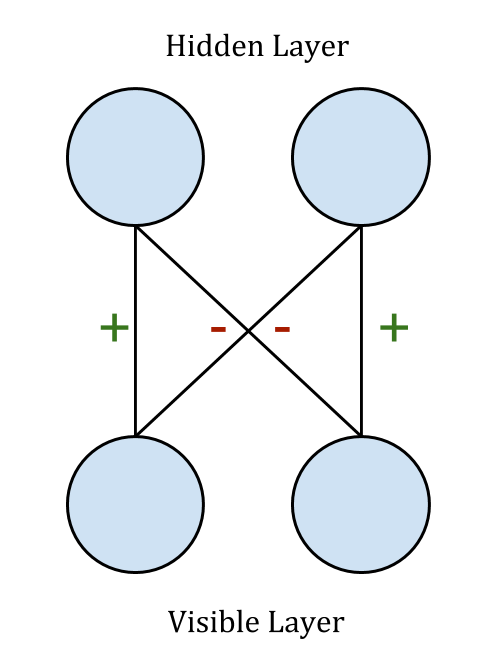
\includegraphics[width=0.3\textwidth]{Assets/Two-Bit-RBM.png}
  \end{center}
  \caption{The two bit RBM for modelling a single bit on at a time in a two bit pattern. The diagonal weights are negative and the non-diagonal weights are positive.}
  \label{F:Two-Bit-RBM}
\end{figure}

\subsubsection{Architecture and Parameters}

\begin{wrapfigure}{l}{0.6\textwidth}
  \begin{center}
    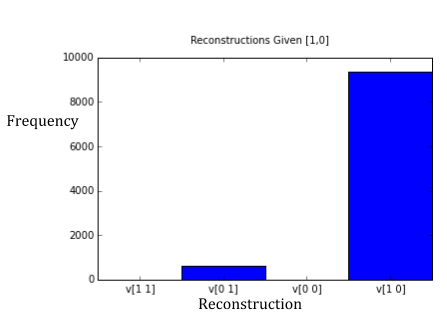
\includegraphics[width=0.5\textwidth]{Assets/Two-Bit-RBM-Recon.png}
  \end{center}
  \caption{Example reconstructions for the Handcrafted RBM, For 10000 independant reconstructions given the input $[1,0]$.}
  \label{F:Two-Bit-RBM-Recons}
\end{wrapfigure}


Being a trivial dimensionality, the RBMs weights were constructed by hand, meaning that only the ORBMs inference algorithm was being evaluated and not the training of the RBMs plugged into it. This network is picture in figure \ref{F:Two-Bit-RBM}, \todowording{with weights greater than 5} the networks stable state results in either $[1 , 0]$ or $[0 , 1]$. The RBMs had 2 hidden units and 2 visible units.

\subsubsection{Method}

This RBM was checked to ensure that it behaved in practice by ensuring it's reconstructions matched the input for a large frequency of reconstructions. With the input $[1,0]$, the results are shown in figure \ref{F:Two-Bit-RBM-Recons}. The most common reconstruction is  $[1,0]$, which matches the input. We see that $~500$ reconstructions out of the $10,000$ reconstructions are incorrect, corresponding to $[0,1]$. This is due to the stochastic nature of the RBM, which is trained to increase the likilyhood of training data, resulting in a small chance of producing reconstructions. This is the why it is important to examine multiple reconstructions, especially in this small dimenionality where taking $10,000$ samples is not time consuming (as it would be in tasks with larger dimensions).
\begin{figure}[!htb]
  \begin{center}
    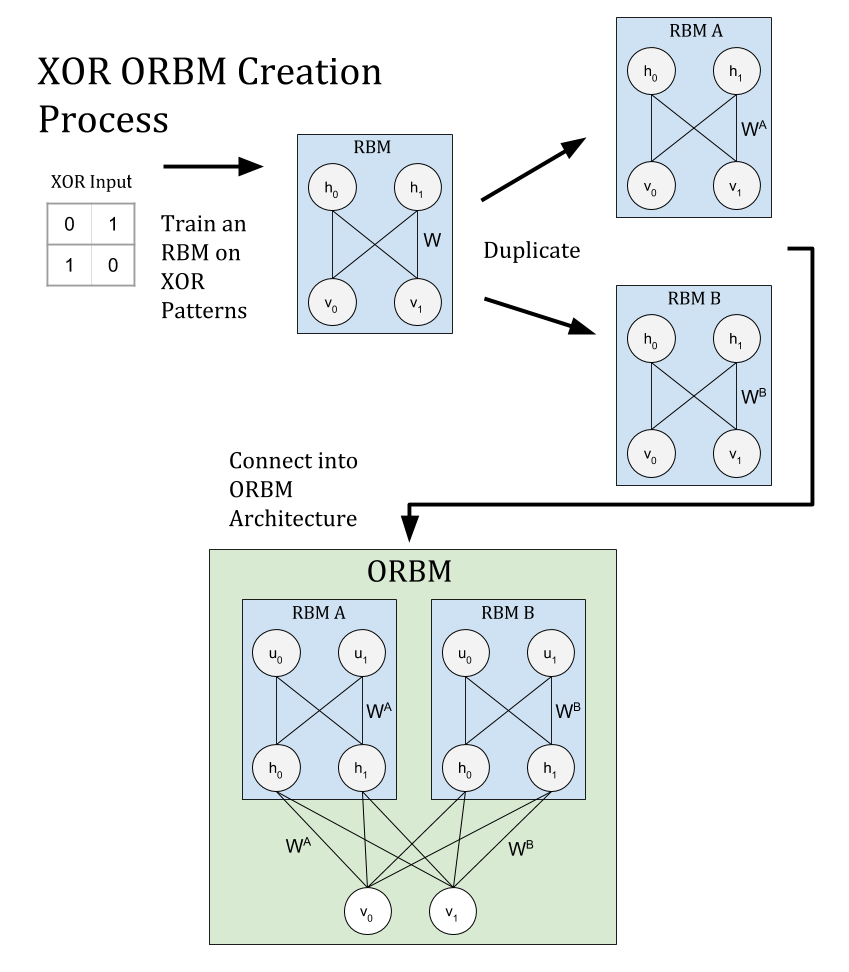
\includegraphics[width=0.7\textwidth]{Assets/XOR-ORBM-Creation-Process.png}
  \end{center}
  \caption{The process used to create the ORBM for evalating composite XOR inputs.}
  \label{F:XOR-ORBM-Creation-Process-Diagram}
\end{figure}

In a similar way to the reconstructions, free-phase visible pattern samples can be taken from the model and evaluated. \todowording{In larger dimensions Hinton has shown RBMs to be poor generative models without the extra layers above...} however in the small dimensions the dreams of the RBM should match the training set. A bar graph of frequencies of dreams is shown in figure \ref{F:Two-Bit-RBM-Dreams}. The RBM behaves as expected, generating dream patterns that match the training set in the correct proportion.
\begin{wrapfigure}{r}{0.4\textwidth}
  \begin{center}
    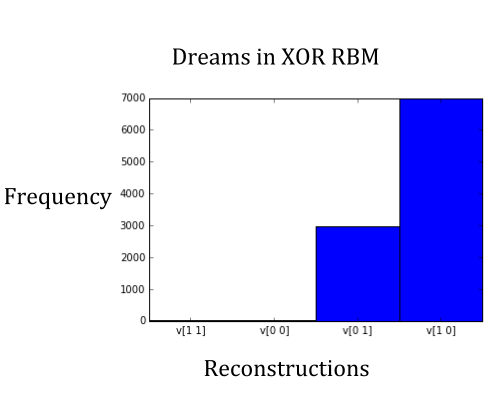
\includegraphics[width=0.35\textwidth]{Assets/XOR-RBM-Dreams.png}
  \end{center}
  \caption{Dreams in the XOR RBM, note how only the training data is present.}
  \label{F:Two-Bit-RBM-Dreams}
\end{wrapfigure}
With a valid model established, the XOR RBM was duplicated and plugged into the ORBM structure as illustrated in Figure \ref{F:XOR-ORBM-Creation-Process-Diagram}.

The inference algorithm was run in the ORBM architecture for various visible inputs, giving two hidden vectors for the two representations $h^A$ and $h^B$. For each pair of hidden vectors, a reconstruction was created, the process illustrated in figure
\begin{figure}[h]
  \begin{center}
    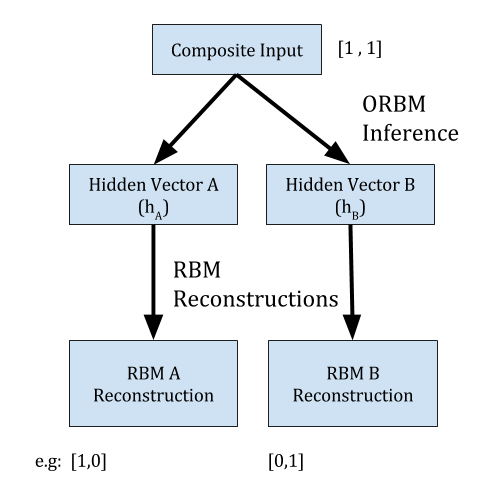
\includegraphics[width=0.5\textwidth]{Assets/XOR-2-Bit-Process-Diagram.png}
  \end{center}
  \caption{The process of generating reconstruction is shown in this diagram.}

  \label{F:Two-Bit-ORBM-Process-Diagram}
\end{figure}
 \ref{F:Two-Bit-ORBM-Process-Diagram}. This process was repeated in a similar way to how the reconstructions were evaluated in the lone RBM, counting the frequency each reconstruction occurred over $1500$ runs.

\begin{table}[]
\centering
\begin{tabular}{|l|l|l|}
\hline
Visible Input & \multicolumn{2}{l|}{Expected Reconstructions} \\ \hline
$[1 , 1 ]$    & $[1, 0]$              & $[0,1]$               \\ \hline
$[1, 0 ]$     & $[1,0]$               & $[1, 0]$              \\ \hline
$[0, 1]$      & $[0,1]$               & $[0,1]$               \\ \hline
\end{tabular}
\caption{A Table showing the expected reconstructions from performing ORBM inference with various input patterns. The left and right hand column of the Expected Reconstructions colummn indicate the reconstructions from the left and right RBMs in the ORBM.}
\label{my-label}
\end{table}

\subsubsection{XOR ORBM Analysis}

The results of this process are shown in figure \ref{F:Two-Bit-ORBM-Inference-Results-1}. Where the x-axis shows the reconstructions of the form A reconstruction, B reconstruction. The results show how applying the full correction compares to the approximated correction.

The ORBM is able to separate the causes with both types of correction, as the model is being duplicated, it produces $[1,0]$ and $[0,1]$ approximately half the time and symetrically $[0,1]\text{ }[1,0]$ the other half of the time. These reconstructions were compared to one of the RBMs trained to recognised a single pattern being on in two bits. As expected a machine that has been trained to recognise one bit, has no concept of two bits being on and hence the reconstructions show no mechanism for seperating the sources. This is illustrated in figure \ref{F:Two-Bit-RBM-Inference-Results-1}.

The results of repeating this process with the input $[1,0]$ yielded successful results. We would hope that ORBM architecture could also handle inference with just a single subject. The results of this are shown in
figure \ref{F:Two-Bit-RBM-Inference-Results-2}.

The ORBM was able to extract the target patterns $[1,0]$ and $[0,1]$ given the input $[1,1]$. This was the case for both the Approximated and Full corrections, which gave confidence that the more computationally efficient Approximated correction could be relied on going forward --- as for larger datasets is was a lot faster in practice. The generative model also copes with the subject overlapping, which in the two bit case arised when $[1,0]$ is composed with $[1,0]$. In both the Approximated and Full corrections the highest occuring reconstruction is the target $[1,0]$, however there appears to be a lot less confidence.


\begin{landscape}
\begin{figure}
  \begin{center}
    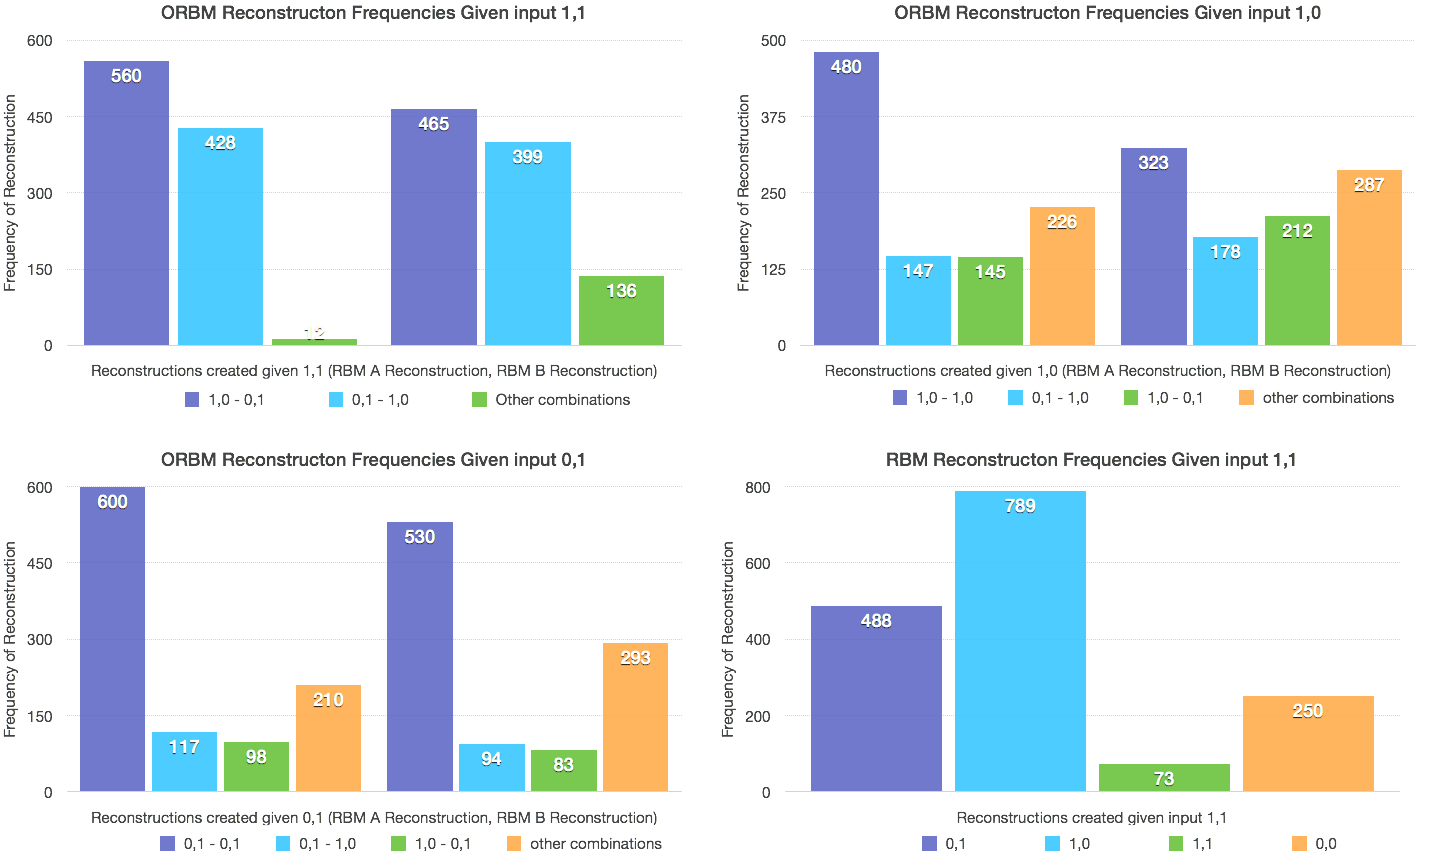
\includegraphics[height=0.9\textheight]{Assets/results/xor-results}
  \end{center}
  \caption{A figure showing the result of generating 1000 reconstructions with an RBM. It is clear the RBM has no mechanism to separate the sources. Hence showing it [1,1] when it has only been trained on XOR results in no separation, i.e. reconstructions including $[1,1]$.}

  \label{F:Two-Bit-RBM-Inference-Results-1}
\end{figure}
\end{landscape}



\section{$Y$ bit pattern, $X$ neighbouring bits on} %%%%%%%%%%%%%%%%%%%%%%%%%%

\subsubsection{Description}
A natural next step from a single bit on in a 2 bit pattern, is moving up to $X$  bits side by side on in a $Y$ bit pattern is a next step. In affect this is modelling a $X$ bit subject, in a $Y$ bit pattern.
For example if $Y = 4 $ and $ X = 2 $ then a valid inputs are the rows of the following table:
\begin{equation}\label{eq:Example-xy-dataset} dataset =
\begin{bmatrix}
  1 & 1 & 0 & 0 \\
  0 & 1 & 1 & 0 \\
  0 & 0 & 1 & 1
\end{bmatrix}
\end{equation}

This allows for some interesting cases, for instance using the same example as above of $Y = 4 $ and $ X = 2 $, we can examine how the ORBM handles separating interesting patterns. For instance where \emph{subjects} partially overlap such as $[1,1,1,0]$, which is a composition of $[1,1,0,0]$ and $[0,1,1,0]$. This evaluation will explore these interesting cases over a subset of the possible combinations of $Y$ and $X$, ensuring that the ORBM is able to reconstuct the combination of images correctly.


\subsubsection{Architecture and Parameters}
\begin{itemize}
  \item $|Y|$ Hidden units per RBM, any less and we were unable to train the RBM to make the target reconstructions or dreams.
  \item Random normally distributed, mean and standard deviation of one, starting weights. The RBM was trained with $1000$ epochs and a learning rate of $0.002$.
  \item A sample of 10,000 dreams were sampled from the RBMs, and then plotted on a histogram in a similar fashion to figure \ref{efnsefskj}. The frequency of produced dreams was ensured to be approximately equal and that the dreams should directly match the training set. This is feasible as the ground truth patterns are known.
\end{itemize}


\subsubsection{Method and Results}

For a subset of values of $y \in Y, x \in X | 2 < x < y < 10$ the following process was repeated:

\begin{enumerate}
  \item A single RBM was trained on all possible permutations of $X$ neighbouring bits being on in a $Y$ bit string (as seen in the Matrix~\ref{eq:Example-xy-dataset}).
  \item The trained RBM was duplicated an plugged into the ORBM architecture.
  \item For a subset of possible compositions of two patterns from xy \todowording{list all combinations for a given xy to show infeasibility of doing them all} generate reconstructions using the ORBM. Where the cases examined are interesting cases such as partial and \todowording{completely overallping and no overlapping}
  \item Plot reconstructions on bar graphs ensuring they match the expected results.
\end{enumerate}

A subset of the larger (but still small) dimension task results are shown in Figure \ref{F:X-Bit-ORBM-Inference-Results-1}. These illustrate the more interesting cases and the ORBM correctly separates the sources in all of them. The top left graph in Figure \ref{F:X-Bit-ORBM-Inference-Results-1} extends the work in section \ref{S:XOR} by recognising a single bit in a 5 bit pattern and the ORBM is sucessful. The top right graph illustrates the case of a 1 bit overlap of data made up of 2 neighbouring bits. The bottom left graph also exemplifies a 1 bit overlay but this time with a `wider` pattern of 3 bits. The bottom right graph shows the case where the two `subjects` are side by side, not overlapping. This is a disparity here that would likely be solved creating more reconstructions.


\begin{landscape}
\begin{figure}
  \begin{center}
    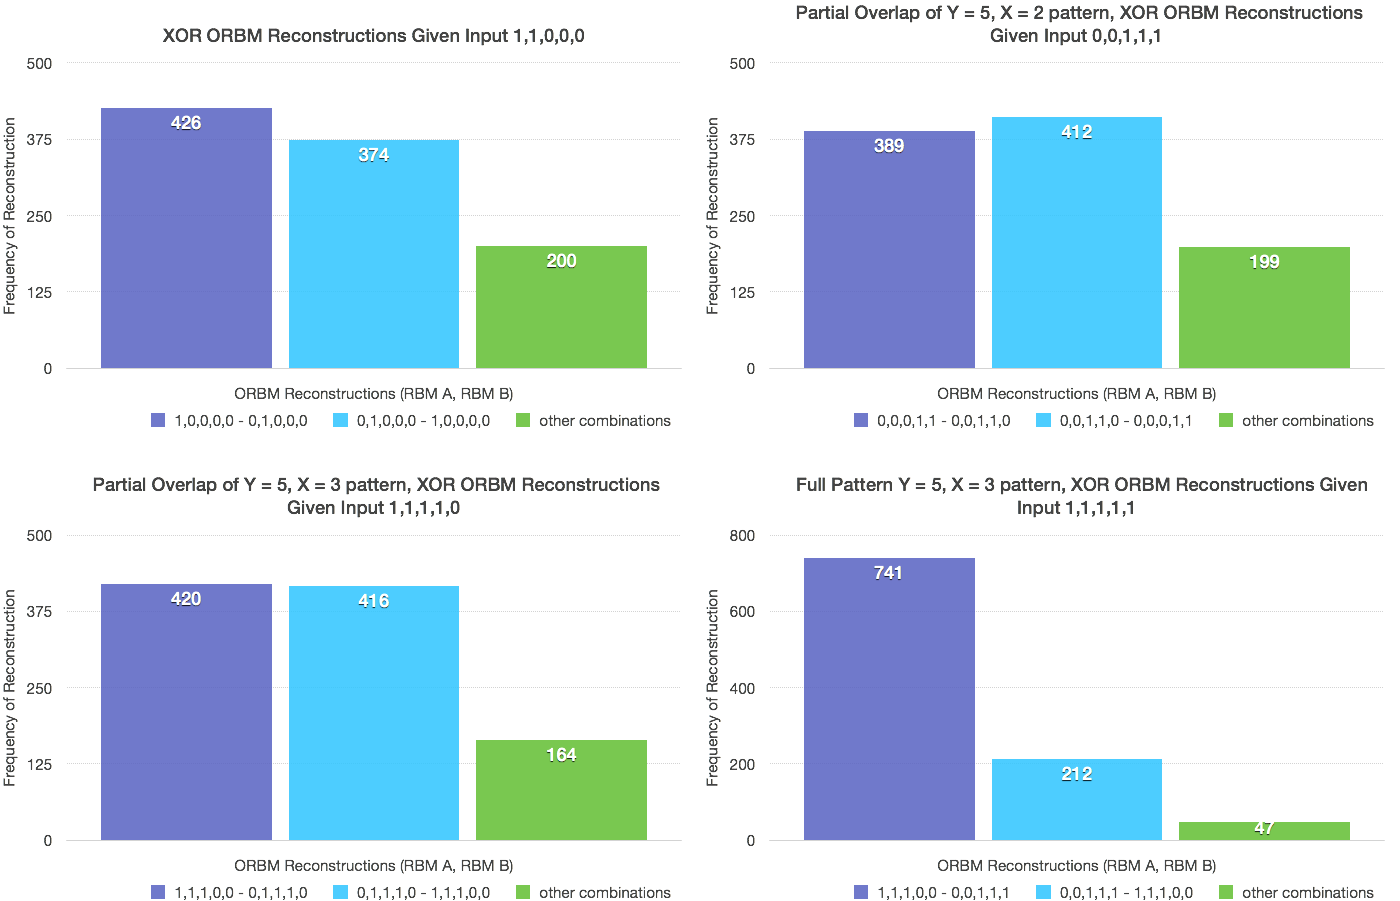
\includegraphics[height=0.9\textheight]{Assets/results/xy-bit-results}
  \end{center}
  \caption{A figure showing interesting cases of ORBM reconstructions in $Y$ bit pattern, $X$ neighbouring bits on.}

  \label{F:X-Bit-ORBM-Inference-Results-1}
\end{figure}
\end{landscape}

\section{2D Patterns in a small dimensional space}%%%%%%%%%%%%%%%%%%%%%%%%%%%%

\subsubsection{Description}
This task continues to work with a single RBM being duplicated, instead increasing the dimensionality from $~10$ to $25$ in the form of a 5 by 5 pixel image. Then another similar model is introduced so the ORBM has to separate a 2 by 2 square and various sized rectangles.

\begin{figure}[htb]
  \begin{center}
    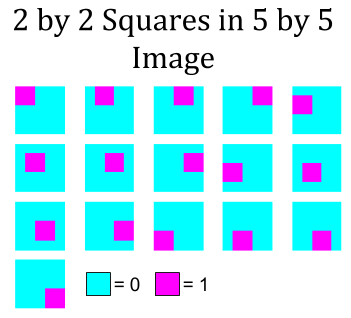
\includegraphics[width=0.3\textwidth]{Assets/results/sq-dataset.png}
  \end{center}
  \caption{A figure illustrating the dataset used for this task. 2 by 2 pixel squares in a 5 by 5 pixel image.}
  \label{F:Sq-Dataset}
\end{figure}

\subsubsection{Architecture and Parameters}
\begin{itemize}
  \item Uses a 25 hidden unit RBM trained on a dataset of every permutation of a 2 by 2 square in a 5 by 5 pixel image. This dataset is illustrated in Figure \ref{F:Sq-Dataset}.
  \item The trained RBMs reconstructions and dreams were visually inspected, as well as Hinton diagrams to ensure an effective model.
  \item When performing inference in the ORBM, 500 Gibbs iterations were used. In practice this number is quite large however as the dimensions are small it is not computational intractable, and this gives more confidence that the ORBM is performing to the best of its ability.
\end{itemize}

\subsubsection{Method and Results}

The method followed a similar process as previous evaluations: Generate the training data and training and verfiying the RBM to make sure it performs well.
Next the whole dataset was composited with every other item in that dataset, and ORBM reconstructions were then generated (using 500 Gibbs iterations when calculating the correction), as were RBM reconstructions.
A subset of compelling results from this process were extracted and are shown in Figure \ref{F:sq-orbm-results}. I only show a single RBM reconstruction here as the same model is being used for both subjects.

\subsubsection{Square results}
\begin{description}
  \item[Column 1] Shows two squares sitting side by side. As expected the RBM, only modelling a single square recontructs a square in the middle of the two. The ORBM is able to successfully extract and reconstruct the separate squares.
  \item[Columns 2 and 3] Here we see a single pixel overlap, the ORBM successfully reconstructing the ground truth. The RBM, despite having identical weights to the RBM that is plugged into the ORBM there is no mechanism to separate the sources. The ORBM does not perform perfectly in column 3, in that one if it's reconstructions is correct but the other is noiser than the RBM.
  \item[Columns 4, 5 and 6] Much like column 1 we have disjoint subjects, the ORBM successfully separates them, however the RBM performs much, much worse.
\end{description}

This process was repeated except a different RBM was introduced, one that represents a rectangle instead of sqaure. Plugging the original square model and the new rectangle into the ORBM architecture. The results for this aspect are shown in \ref{F:rect-orbm-results}.

\subsubsection{Rectangle results}
\begin{description}
  \item[Columns 1 and 2] These show two instances of the ORBM being able to separate a square and rectangle of different sizes.
  \item[Columns 3] This shows a confusing case where the square is completely occluded by the the larger square. The ORBM reconstructions look valid in that it reconstructs the correct shapes, unlike the RBM, however the placing of the 2 by 2 square is in fact incorrect.
  \item[Columns 4, 5 and 6] Here we see partially overlapping shapes of various sizes. The ORBM generates less noisy reconstructions compared to the RBM.
\end{description}




\begin{figure}[htb]
  \begin{center}
    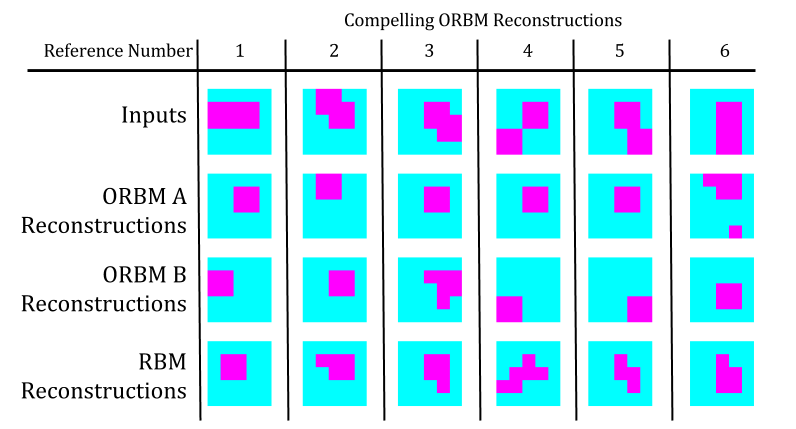
\includegraphics[width=\textwidth]{Assets/results/sq-orbm-results.png}
  \end{center}
  \caption{Figure illustrating a subset of the the results from ORBM inference on 2 By 2 square images.}
  \label{F:sq-orbm-results}
\end{figure}

\begin{figure}[htb]
  \begin{center}
    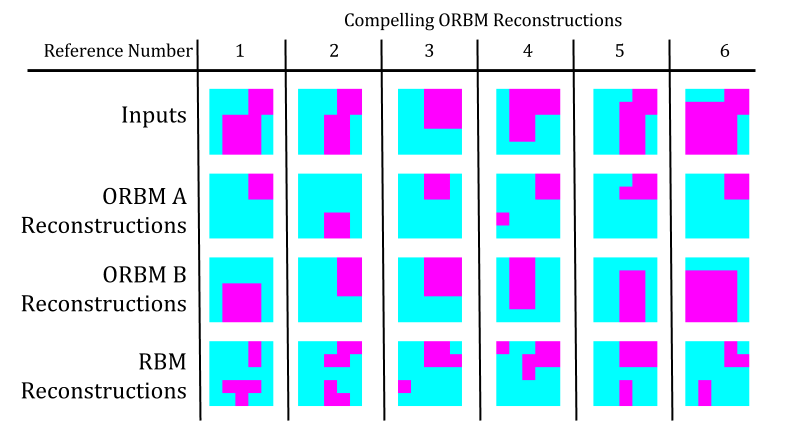
\includegraphics[width=\textwidth]{Assets/results/rect-sq-orbm-results.png}
  \end{center}
  \caption{Figure illustrating a subset of the the results from ORBM inference on 2 by 2 squares combined with $x$ by $y$ pixel rectangles. Note that there is a different RBM (and corresponding ORBM) being used for different values of $x$ and $y$ in the figure.}
  \label{F:rect-orbm-results}
\end{figure}


  \section{MNIST Digits Mixing Time and Reconstructions}

  \subsubsection{Description}
  MNIST is a widely used dataset of handwritten digits (0 -- 9). This evaluation explored the non-trivial task of given two handwritten digits composited to form one image, how effectively can the ORBM separate the sources compared to the naive RBM? An example input is illustrated in figure \todocite{\ref{}}.

  \subsubsection{Architecture and Parameters}

  \begin{itemize}
    \item MNIST Digit images are 28 by 28 pixel images, with pixel values between 0 -- 1.
    \item Ten RBMs each with 100 Hidden units trained on 500 examples of each digit respectively. Reconstructions and dreams of these RBMs were inspected by hand to ensure that they resembled the dataset.
  \end{itemize}

  \subsubsection{Method and Results}

  For every digit dataset (of size 500), each digit in each dataset was composed with every other digit in every other dataset. Given this set of composite datasets, the corresponding RBMs were plugged in the ORBM architecture and used to create reconstructions.

  As an MNIST image has 784 (28 by 28 pixels) features, more consideration is need for how many Gibbs iterations should be used to generate the hidden states ($h^A$ and $h^B$) given the input. By examining reconstructions at different points in the Gibbs chain we can get a sense of how quickly the chain is mixing. A subset of these chains are illustrated in Figure \ref{F:MNIST-Mixing-Time}.
  \begin{figure}[htb]
    \begin{center}
      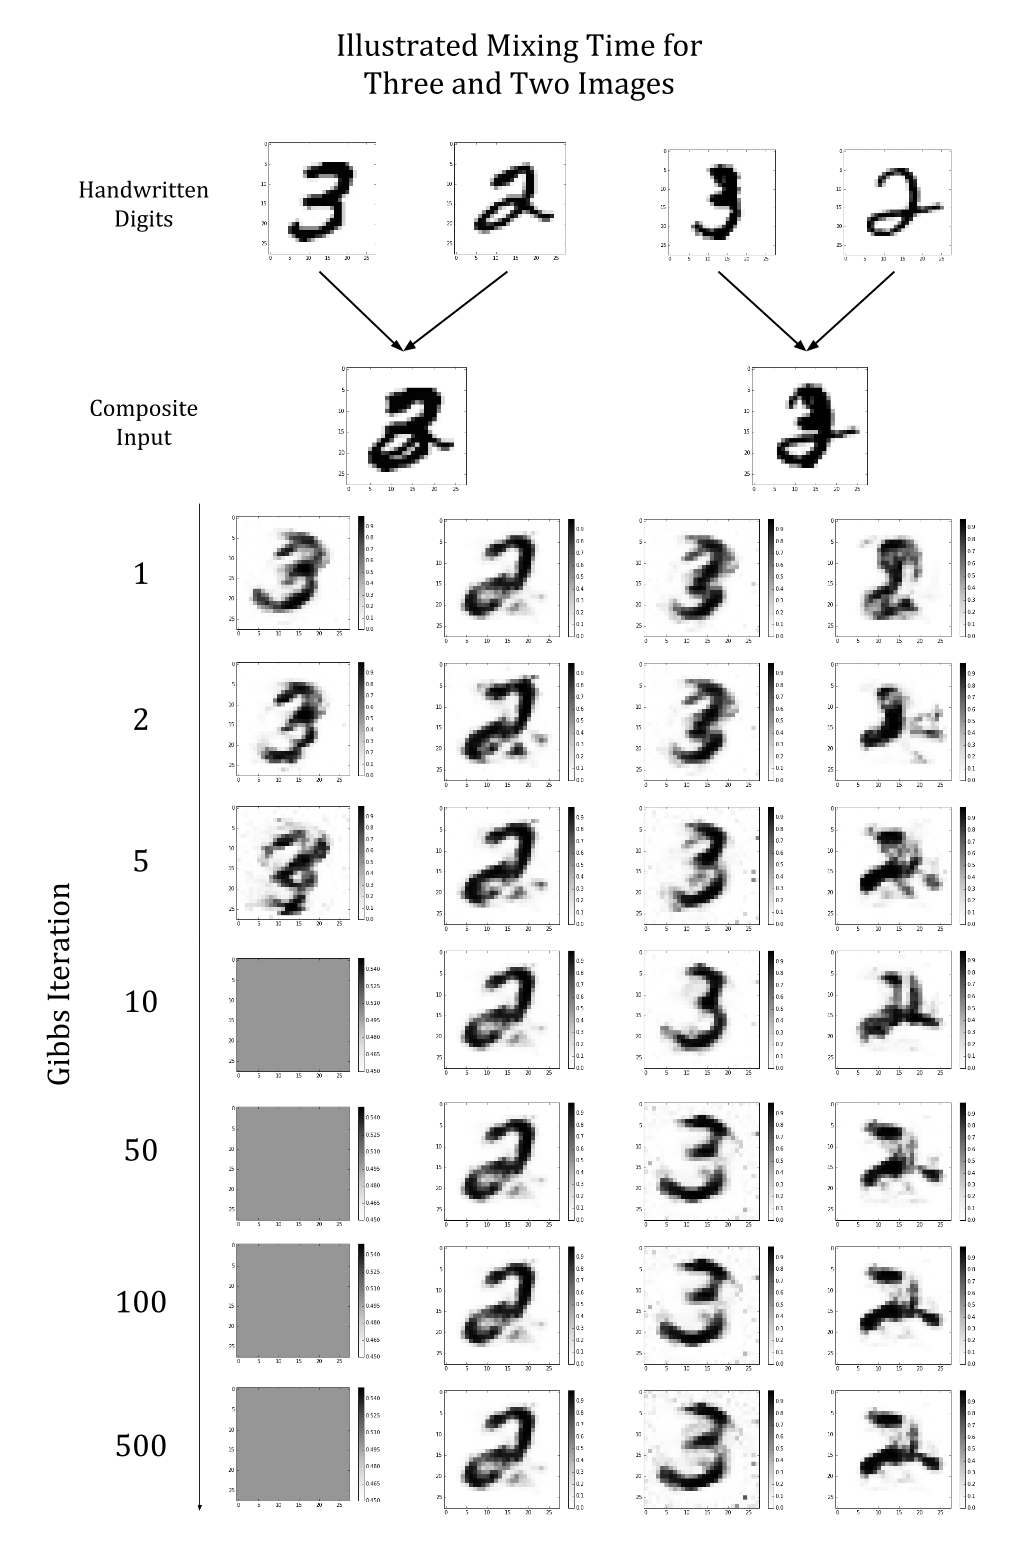
\includegraphics[width=0.8\textwidth]{Assets/results/Mixing-Results.png}
    \end{center}
    \caption{A figure visualising how reconstructions change in the ORBM as Gibbs iterations are run for two compositions of digits three and two.}
    \label{F:MNIST-Mixing-Time}
  \end{figure}
  By visiually inspecting the reconstructions and the associated hidden activations (the hidden activations are not pictured) at Gibbs iterations 1,2,5,10,50,100, and 500 it can be seen the Gibbs chain mixes very quickly. Viewing these reconstructions as animations it is easier to see how the reconstructions stabilise and this lead to the choice of 100 Gibbs iterations, just to be enusre the chain is definitly mixed while not being such a long chain that it is intractbale to run.

  This diagram also reveals an interesting case where the hidden activations have turned completley off. The reconstruction however appears grey with all values pixel being $0.5$. As mentioned in Section \todocite{where are the biases\ref{}} the ORBM does not use a visible bias which would be responsibile for making an all zero reconstruction given no activations in the hidden layer.


  Given the results of the exploration of the mixing time, 100 Gibbs iterations were used when generating the hidden states ($h^A$ and $h^B$) for a given input. The RBMs plugged into the ORBM were also used to create standard RBM reconstructions, to compare against the ORBM. Given the ORBMs reconstructions (two per image) and the RBM reconstructions (also two per image), two scores were applied to compare these reconstructions to the ground truth:
  \begin{description}
    \item[Cross Entropy] The cross entropy was calculated between the reconstruction and the ground truth.
    \item[Cosine Angle] The angle between the flattened reconstruction vectors was computed, then negated to give a `score`. The higher the score the smaller the angle between the reconstruction vector and the ground truth.
  \end{description}
  These scores can then be summed over each digit and over the entire dataset to find a single score for each digit composed with every other digit forming a 9 by 9 matrix. A cell of this matrix (say $j,i$) corresponds to the difference between the ORBM score and RBM scores for digits $j$ and $i$ composited together. This entire process was repeated 10 times gain certainty in the results --- given the stochasticity of the RBM and ORBM. This process is shown in Algorithm \ref{alg:scores}.

  \begin{algorithm}[!ht]
   \KwData{MNIST Digit datasets, each with 500 examples, 10 RBMs trained on MNIST data 0--9 respectively}
   \KwResult{Composite Datasets for every digit}

   \For {10 repetitions to gain confidence in results} {
     \For{All MNIST digits datasets}{
      \For{Every digit example in the MNIST digit}{
        composite the current digit dataset with every other dataset\;
        Generate reconstructions on that dataset using the ORBM, RBM\;
        Calculate the Cosine Angle score and Cross Entropy for both the RBM's and ORBM's reconstructions versus the ground truth\;
      }
      Sum the scores over every digit example\;
     }
     Tabulate the summed scores in a several matrices indexed by the digits being composited\;
   }
  \caption{The algorithm explaining how the scores matrices were computed.}\label{alg:scores}
  \end{algorithm}

  By finding the difference between the ORBMs reconstructions and the RBMs reconstruction we can create another matrix, in which a positive value represents a `win` for the ORBMs reconstructions and a negative value represents a `loss` (where the RBM outperformed the ORBM).

  \subsubsection{Results}
  These score difference matrices are seen in for the Cross Entropy and Cosine Angle scores in \ref{F:Cross-Entropy-MNIST} and \ref{F:Cosine-MNIST} respectively, where the colour encodes the score. For the Cosine score,  using the approximate correction, zero composed with every other digit yielded the best results for ORBM relative to the RBM, and nine the converse yielding particularly bad results (worse by a factor of 10 compared to zero). Given this, I plotted the RBMs Score versus the ORBM Score as a scatter plot, where each point corresponds to a score. This allows us to examine if the ORBM is performing worse as a whole, or if in some cases it is performing better than the RBM. These plots for zero and nine are shown in \ref{fig:mnist-worse-best-results}.
  \begin{figure}[h]
  \centering
  \begin{subfigure}[t]{0.45\textwidth}
      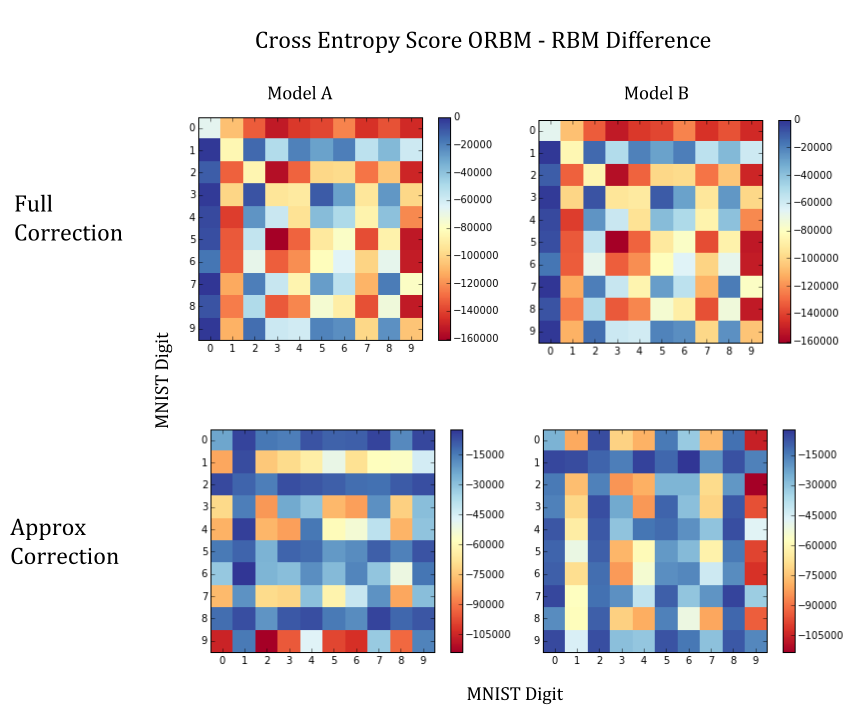
\includegraphics[width=\textwidth]{Assets/Cross-Entropy-Score.png}
      \caption{The cross entropy score summed over every item in the composite dataset.}
      \label{F:Cross-Entropy-MNIST}
  \end{subfigure}
  ~ %add desired spacing between images, e. g. ~, \quad, \qquad, \hfill etc.
    %(or a blank line to force the subfigure onto a new line)
  \begin{subfigure}[t]{0.45\textwidth}
      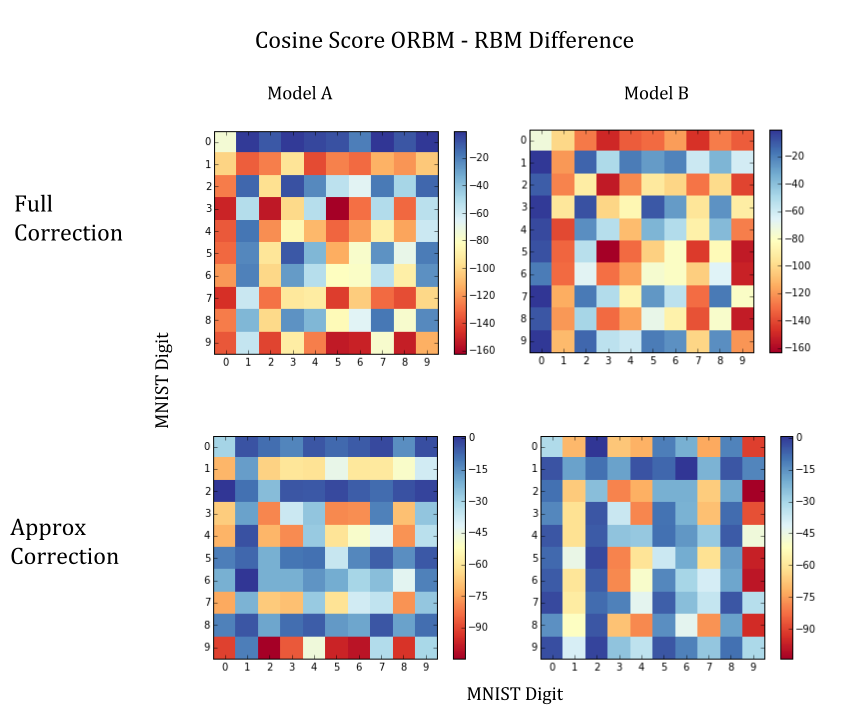
\includegraphics[width=\textwidth]{Assets/Cosine-Score.png}
      \caption{The cosine score summed over every item in the composite dataset.}
      \label{F:Cosine-MNIST}
  \end{subfigure}
  \caption{Dataset-wide MNIST Score Results }\label{fig:mnist-dataset-wide-results}
\end{figure}

\begin{figure}[h]
    \centering
    \begin{subfigure}[t]{1\textwidth}
        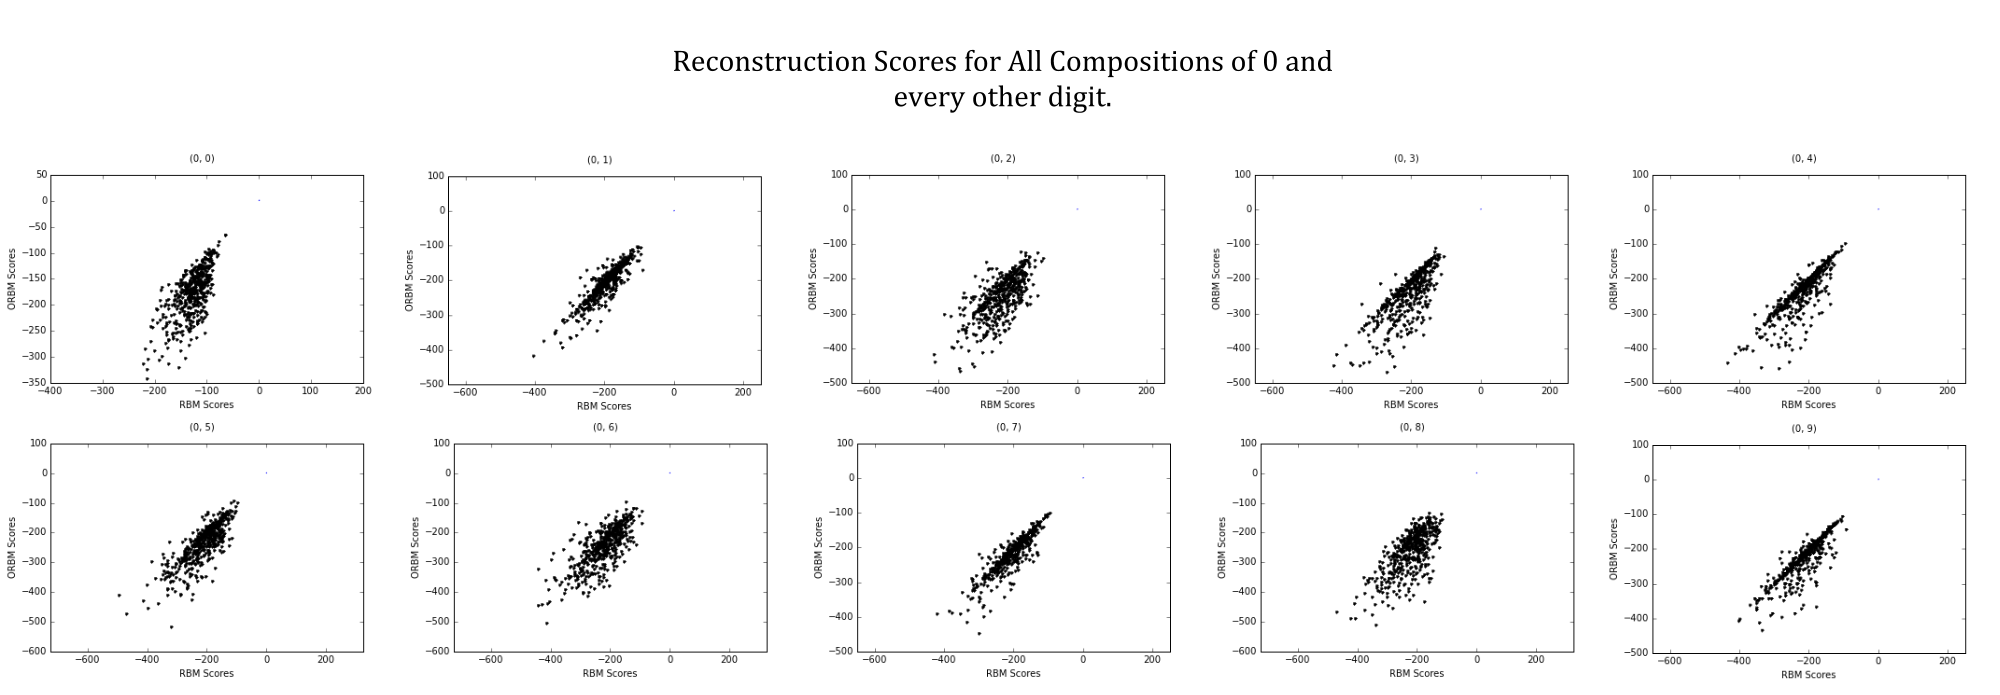
\includegraphics[width=\textwidth]{Assets/b.png}
        \caption{ $(0,x)$ }
      \label{F:Cosine-0-x-scores}
    \end{subfigure}
    \begin{subfigure}[t]{1\textwidth}
        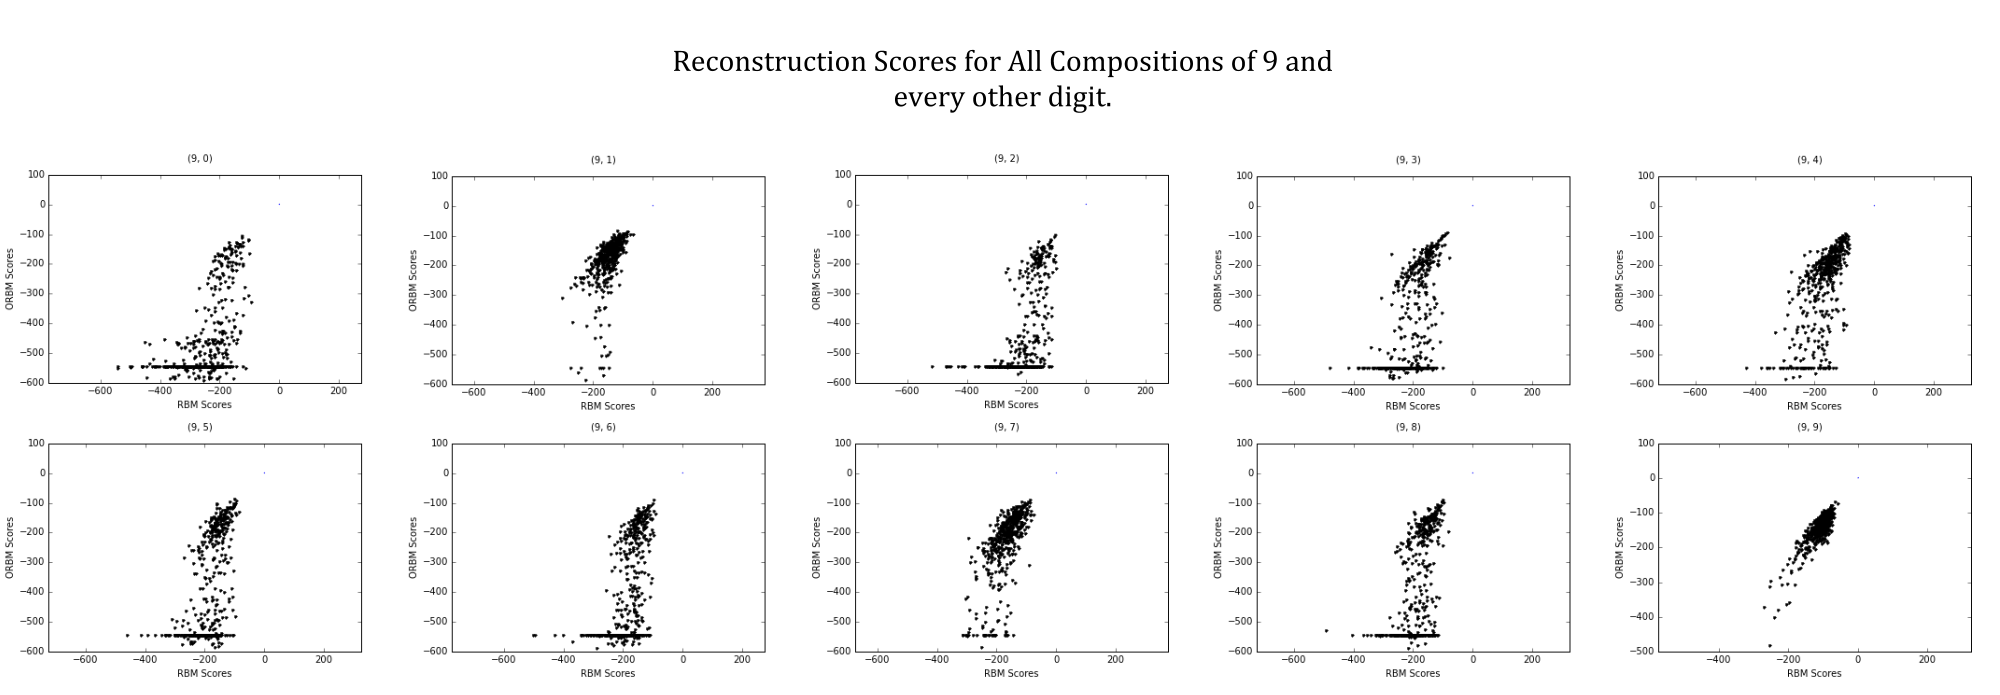
\includegraphics[width=\textwidth]{Assets/(9,X)-ReconstructionScores.png}
        \caption{ $(9,x)$ }
      \label{F:Cosine-9-x-scores}
    \end{subfigure}
    \caption{Cosine Score breakdown for the highest and lowest performing datasets, 0 and 9.}\label{fig:mnist-worse-best-results}
\end{figure}

\begin{figure}[htb]
  \begin{center}
    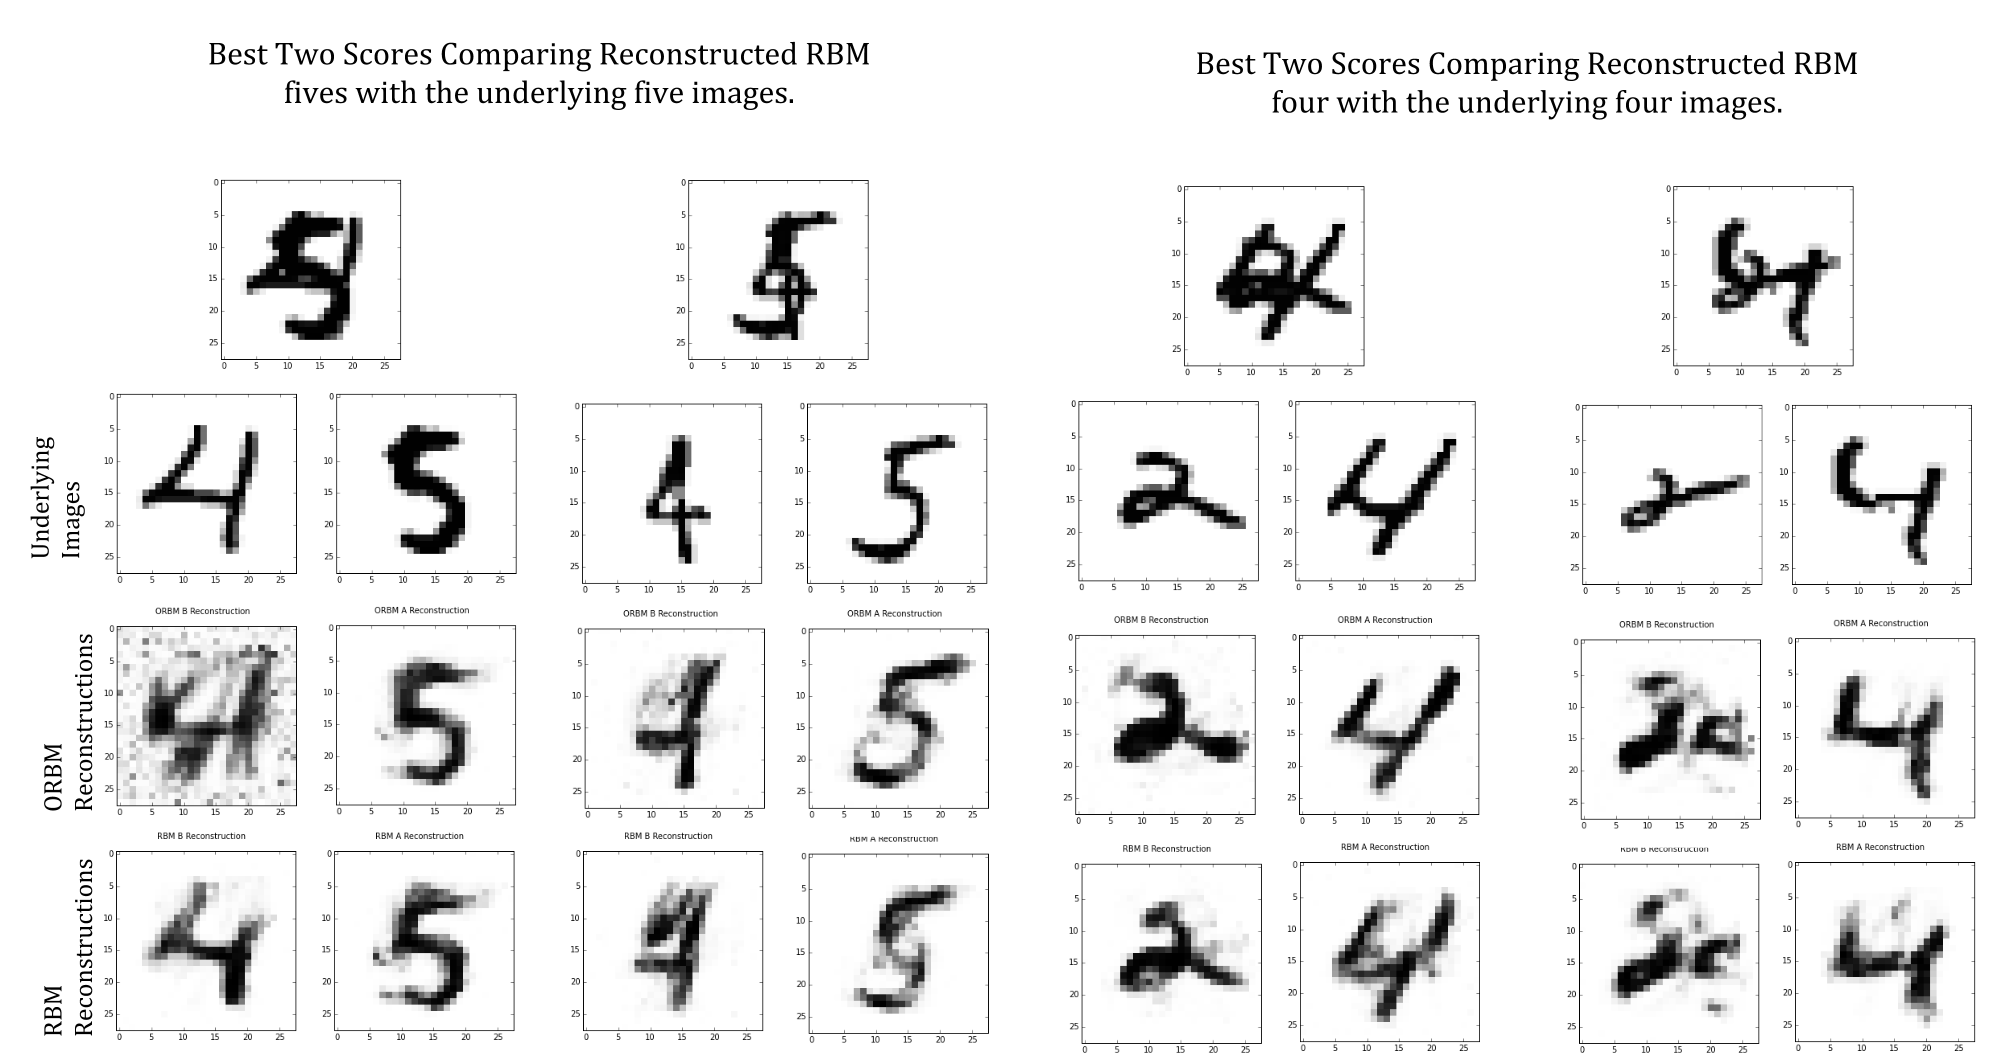
\includegraphics[width=0.9\textwidth]{Assets/results/orbm-Best-2-results.png}
  \end{center}
  \caption{Best Scores}
  \label{F:Best-Results-MNIST}
\end{figure}

\begin{figure}[htb]
  \begin{center}
    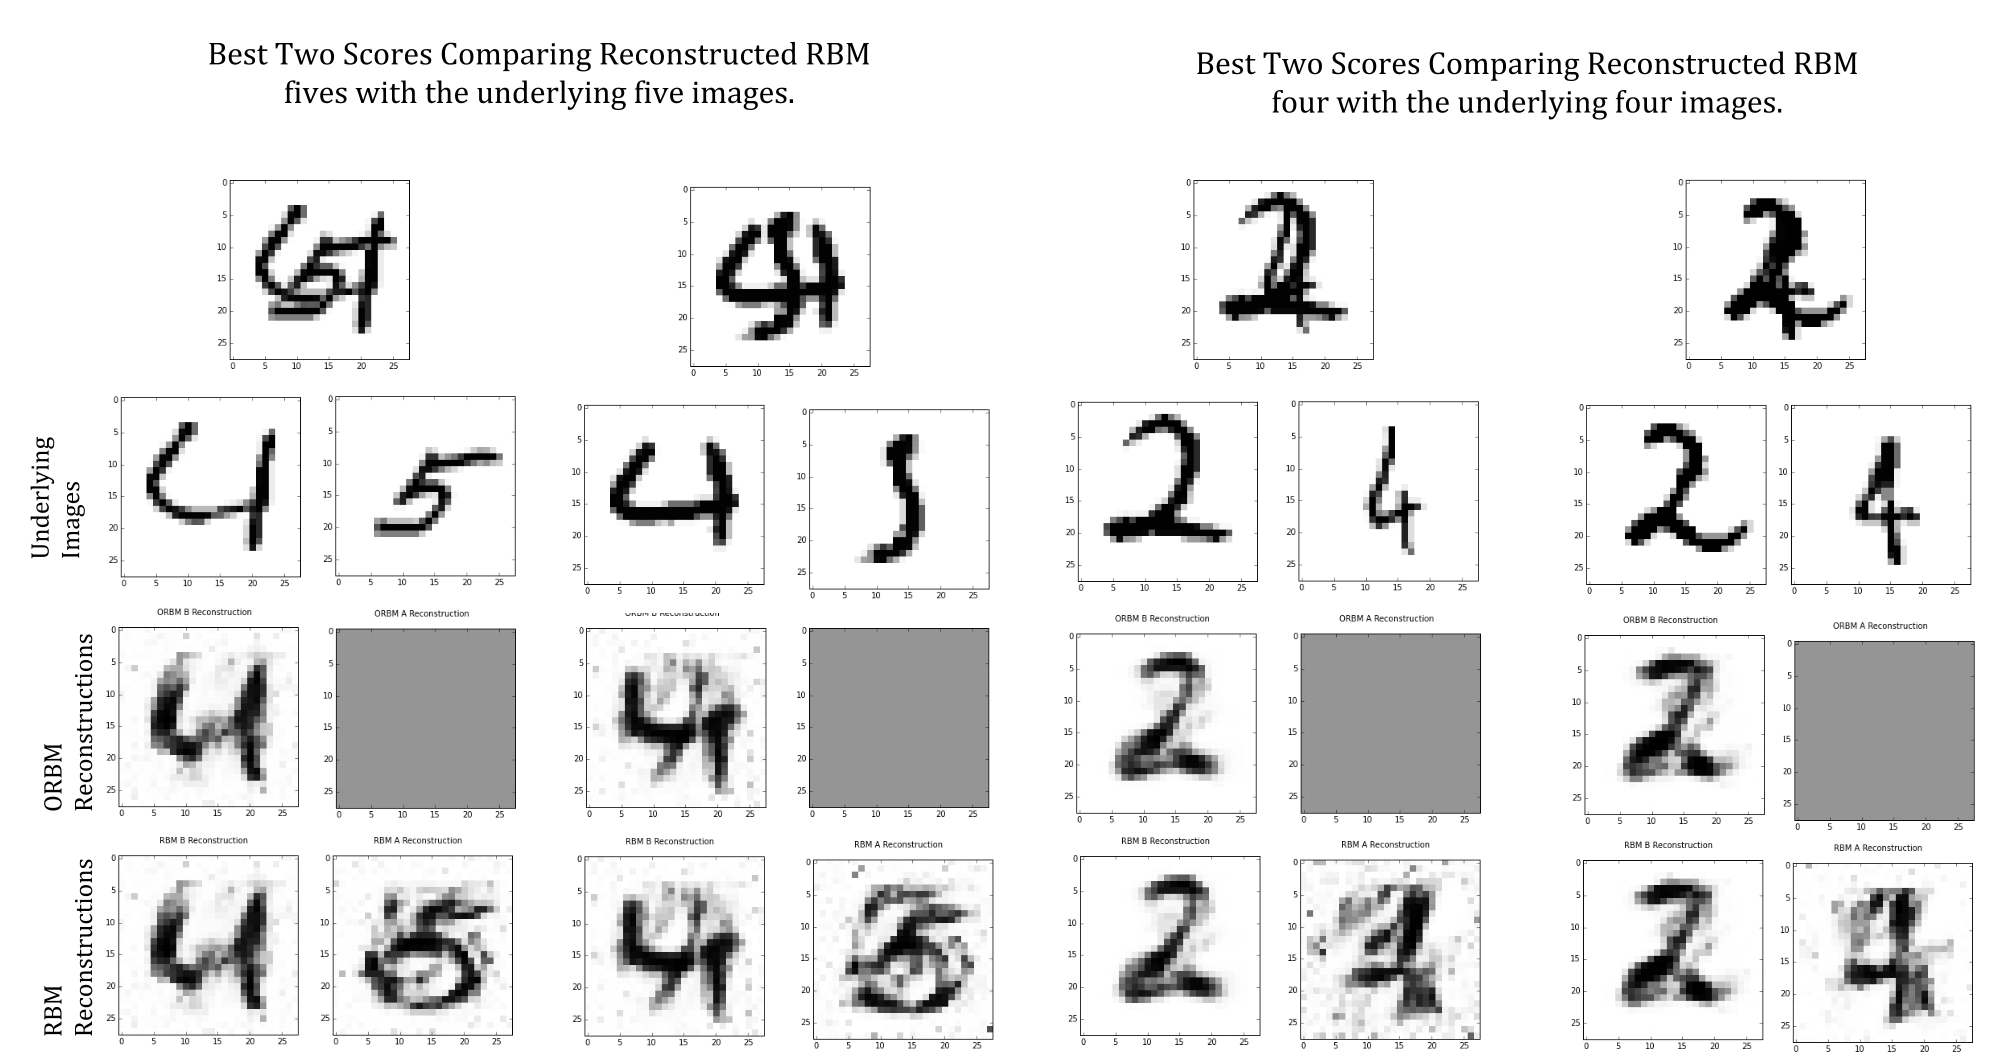
\includegraphics[width=0.9\textwidth]{Assets/results/orbm-Worst-2-results.png}
  \end{center}
  \caption{Worst Scores}
  \label{F:Worst-Results-MNIST}
\end{figure}


\subsection{MNIST Analysis}

It is clear that RBM has better scores than the ORBM when summed over the dataset, and surprising the Approximated correction results in better scores than the Full Correction calculation. For the dataset wide scores \ref{fig:mnist-dataset-wide-results} I would expect to see symmetry in that, for example four composited with five, should score the same as five composited with four.
This asymmetry was not present in the smaller cases, so it was important to examine the RBM and ORBM scores for individual training images \todocite{\ref{}}. In the


\section{Evaluation Analysis}

It is clear that the ORBM outperforms the RBM in source seperation in the smaller tasks, such as XOR. However, as the size of the problems increased I had less confidence until ultimately it performed worse by the scores defined in the MNIST digit dataset. This amounts to the inference algorithm performing worse in large dimenions, with harder tasks. It is not related to the mixing time as that was explored on the same task that the ORBM had the most trouble with. In fact in examining the mixing time it appears it takes very few Gibbs iterations to actually arrive and settle at the wrong answer \todocite{\ref{}}.
Yet in examining \todocite{\ref{}} the individual scores for the various compositions of the MNIST dataset, the ORBM is performing worse in the majority of cases with only a small subset of examples scoring better than the RBM acting alone. Yet looking at example reconstructions \todocite{, as illustrated in \ref{}} I would not say that it is that clear cut that the ORBM is performing worse.

As possible explaination could be that by plugging seporately traineded RBMs, into the ORBM architecture means that there is no regularisation of weights between the two RBMs. The RBMs were trained independantly until they produced accurate reconstructions and dreams that approximately matched items from the dataset, however the process was adhoc and not identical per model. The reason this could be an issue is that the correction adjusts the visible input to the other model by roughly the weight. If the range of weights between the models is drastically different then one model could ``overpower'' the other. This would explain the effect illustrated in the \todocite{worst scoring images of the ORBM pictured in Figure \ref{}} where one of the hidden representations generated is entirely zero (no activation) as the other RBM is ``taking responsibility'' for the input.
    % \begin{itemize}
    %   \item Dataset
    %   \begin{itemize}
    %     \item 500, 28 by 28 pixel, 0-1 valued, handwritten digit images form the training set.
    %   \end{itemize}
    %   \item Method
    %   \begin{itemize}
    %     \item Train an single RBM per digit (0-9) in the dataset. Each RBM having 100 hidden units, (TODO-CITE-COOKBOOK) for reasoning.
    %     \item For all 500 training digit images, compose it with every other digit, and itself. This way the ground truth, the sources are known, therefore making evaluation possible.
    %     \item For all of these compositions us the RBMs trained of the corresponding sources to:
    %     \begin{itemize}
    %       \item Compute the RBM reconstructions for the two sources given their composite input. (TODO-SHOW-DIAGRAM)
    %       \item Compute the ORBM reconstructions, the ORBM using the same RBMs as in the RBM evaluation.
    %       \item Because 28 by 28 pixels equates to 784 features, emperically examining all reconstructions is non-trivial. Hence some scoring functions are required.
    %       \item Scoring
    %       \item Cross Entropy - Approximate the Log likelihood of the underlying dataset.
    %       \item Pixel Difference Score - Absolute difference in pixels of the image
    %       \item Cosine Angle - between reconstruction and target vectors. This has the benefit of also being somewhat magnitude agnostic. (TODO-CITE-AS-MEASURE-WITH-JUSTIFICATION).
    %       \item Repeat this process 30x to give confidence in findings. Scores calculated can then be meaned over the 30 runs.
    %     \end{itemize}
    %   \end{itemize}
    % \end{itemize}



%   \begin{itemize}
%     \item Method
%     \item Can check the inference algorithm by using RBMs with hand trained weights
%     \item Using a single RBM, copied.
%     \item Diagram with small explaination why RBMs with these weights will work.
%     \begin{itemize}
%       \item 2 Hidden Units, 2 Visible Units. Weights Matrix of [-1,1],[1,-1]
%       \item This ensures that if one visible unit is 1, the other will get set to off.
%     \end{itemize}
%     \item Look at the reconstructions of these RBMs, should match XOR patterns.
%     \begin{itemize}
%       \item 100000 free phase samples from RBMs resulted in [1,0] and [0,1] most of the time. (TODO-SHOW-GRAPHs). 100000 free phase samples is quite quick to calculate for only 4 weights.
%       \item 2 sets of 100000 reconstructions given the patterns [1,0] and [0,1] resulted in all reconstructions for each set producing [1,0] and [0,1].
%     \end{itemize}
%     \item Hypothesis
%     \item Clamp the visible to patterns of interest. Can see the dynamics of the system.
%     \begin{itemize}
%       \item 1,1 This should result in reconstructions matching XOR - [1,0] and [0,1]
%       \item 1,0 This should result in reconstructions of just - [1,0]
%       \item 0,1 Should behave symmertrically to [1,0].
%       \item 0,0 Under the dynamics of the generative model should fall into [0,0].
%     \end{itemize}
%   \end{itemize}
%
%   \subsection{Y Bit pattern, X bits On}
%   \begin{itemize}
%     \item Have to train an RBM to recognise X neighbouring bits on at a time in a Y bit pattern. e.g. X = 2, Y = 5, [0,0,1,1,0]
%     \item num Y hiddens, or more.
%     \item While Y less than 10 it is easy to visualise if separation is occurring.
%   \end{itemize}
%
%   \subsection{2D Pattern, Square Separation, Single Model}
%   \begin{itemize}
%     \item Dataset:
%     \begin{itemize}
%       \item 2x2 square in a 5x5 image. Dataset of every possible configuration of said square.
%     \end{itemize}
%     \item Method:
%     \begin{itemize}
%       \item train a single RBM to represent 2x2 squares in 5x5 space. Nice and small, can still inspect reconstructions, and dreams.
%       \item Compose two square images with each other, can the ORBM architecture separate the images.
%     \end{itemize}
%   \end{itemize}
%
%   \subsection{2D Pattern, Different Rectangle Separation}
%   \begin{itemize}
%     \item Dataset
%     \begin{itemize}
%       \item n by m rectangles in 5x5 Images (TODO-IMAGE-IN-HERE) where n and m are not always equal.
%     \end{itemize}
%     \item Method
%     \begin{itemize}
%       \item Superimpose two images as the same way as before. How well can they separate.
%     \end{itemize}
%   \end{itemize}
%
%   \subsection{MNIST Digits}
%   \begin{itemize}
%     \item Dataset
%     \begin{itemize}
%       \item 500, 28 by 28 pixel, 0-1 valued, handwritten digit images form the training set.
%     \end{itemize}
%     \item Method
%     \begin{itemize}
%       \item Train an single RBM per digit (0-9) in the dataset. Each RBM having 100 hidden units, (TODO-CITE-COOKBOOK) for reasoning.
%       \item For all 500 training digit images, compose it with every other digit, and itself. This way the ground truth, the sources are known, therefore making evaluation possible.
%       \item For all of these compositions us the RBMs trained of the corresponding sources to:
%       \begin{itemize}
%         \item Compute the RBM reconstructions for the two sources given their composite input. (TODO-SHOW-DIAGRAM)
%         \item Compute the ORBM reconstructions, the ORBM using the same RBMs as in the RBM evaluation.
%         \item Because 28 by 28 pixels equates to 784 features, emperically examining all reconstructions is non-trivial. Hence some scoring functions are required.
%         \item Scoring
%         \item Cross Entropy - Approximate the Log likelihood of the underlying dataset.
%         \item Pixel Difference Score - Absolute difference in pixels of the image
%         \item Cosine Angle - between reconstruction and target vectors. This has the benefit of also being somewhat magnitude agnostic. (TODO-CITE-AS-MEASURE-WITH-JUSTIFICATION).
%         \item Repeat this process 30x to give confidence in findings. Scores calculated can then be meaned over the 30 runs.
%       \end{itemize}
%     \end{itemize}
%   \end{itemize}
%
%
% % \subsection{Classifciation Accuracy on Hidden Representation}
% %   Not sure about this one.
